% Options for packages loaded elsewhere
\PassOptionsToPackage{unicode}{hyperref}
\PassOptionsToPackage{hyphens}{url}
%
\documentclass[
]{article}
\usepackage{amsmath,amssymb}
\usepackage{iftex}
\ifPDFTeX
  \usepackage[T1]{fontenc}
  \usepackage[utf8]{inputenc}
  \usepackage{textcomp} % provide euro and other symbols
\else % if luatex or xetex
  \usepackage{unicode-math} % this also loads fontspec
  \defaultfontfeatures{Scale=MatchLowercase}
  \defaultfontfeatures[\rmfamily]{Ligatures=TeX,Scale=1}
\fi
\usepackage{lmodern}
\ifPDFTeX\else
  % xetex/luatex font selection
\fi
% Use upquote if available, for straight quotes in verbatim environments
\IfFileExists{upquote.sty}{\usepackage{upquote}}{}
\IfFileExists{microtype.sty}{% use microtype if available
  \usepackage[]{microtype}
  \UseMicrotypeSet[protrusion]{basicmath} % disable protrusion for tt fonts
}{}
\makeatletter
\@ifundefined{KOMAClassName}{% if non-KOMA class
  \IfFileExists{parskip.sty}{%
    \usepackage{parskip}
  }{% else
    \setlength{\parindent}{0pt}
    \setlength{\parskip}{6pt plus 2pt minus 1pt}}
}{% if KOMA class
  \KOMAoptions{parskip=half}}
\makeatother
\usepackage{xcolor}
\usepackage[margin=1in]{geometry}
\usepackage{color}
\usepackage{fancyvrb}
\newcommand{\VerbBar}{|}
\newcommand{\VERB}{\Verb[commandchars=\\\{\}]}
\DefineVerbatimEnvironment{Highlighting}{Verbatim}{commandchars=\\\{\}}
% Add ',fontsize=\small' for more characters per line
\usepackage{framed}
\definecolor{shadecolor}{RGB}{248,248,248}
\newenvironment{Shaded}{\begin{snugshade}}{\end{snugshade}}
\newcommand{\AlertTok}[1]{\textcolor[rgb]{0.94,0.16,0.16}{#1}}
\newcommand{\AnnotationTok}[1]{\textcolor[rgb]{0.56,0.35,0.01}{\textbf{\textit{#1}}}}
\newcommand{\AttributeTok}[1]{\textcolor[rgb]{0.13,0.29,0.53}{#1}}
\newcommand{\BaseNTok}[1]{\textcolor[rgb]{0.00,0.00,0.81}{#1}}
\newcommand{\BuiltInTok}[1]{#1}
\newcommand{\CharTok}[1]{\textcolor[rgb]{0.31,0.60,0.02}{#1}}
\newcommand{\CommentTok}[1]{\textcolor[rgb]{0.56,0.35,0.01}{\textit{#1}}}
\newcommand{\CommentVarTok}[1]{\textcolor[rgb]{0.56,0.35,0.01}{\textbf{\textit{#1}}}}
\newcommand{\ConstantTok}[1]{\textcolor[rgb]{0.56,0.35,0.01}{#1}}
\newcommand{\ControlFlowTok}[1]{\textcolor[rgb]{0.13,0.29,0.53}{\textbf{#1}}}
\newcommand{\DataTypeTok}[1]{\textcolor[rgb]{0.13,0.29,0.53}{#1}}
\newcommand{\DecValTok}[1]{\textcolor[rgb]{0.00,0.00,0.81}{#1}}
\newcommand{\DocumentationTok}[1]{\textcolor[rgb]{0.56,0.35,0.01}{\textbf{\textit{#1}}}}
\newcommand{\ErrorTok}[1]{\textcolor[rgb]{0.64,0.00,0.00}{\textbf{#1}}}
\newcommand{\ExtensionTok}[1]{#1}
\newcommand{\FloatTok}[1]{\textcolor[rgb]{0.00,0.00,0.81}{#1}}
\newcommand{\FunctionTok}[1]{\textcolor[rgb]{0.13,0.29,0.53}{\textbf{#1}}}
\newcommand{\ImportTok}[1]{#1}
\newcommand{\InformationTok}[1]{\textcolor[rgb]{0.56,0.35,0.01}{\textbf{\textit{#1}}}}
\newcommand{\KeywordTok}[1]{\textcolor[rgb]{0.13,0.29,0.53}{\textbf{#1}}}
\newcommand{\NormalTok}[1]{#1}
\newcommand{\OperatorTok}[1]{\textcolor[rgb]{0.81,0.36,0.00}{\textbf{#1}}}
\newcommand{\OtherTok}[1]{\textcolor[rgb]{0.56,0.35,0.01}{#1}}
\newcommand{\PreprocessorTok}[1]{\textcolor[rgb]{0.56,0.35,0.01}{\textit{#1}}}
\newcommand{\RegionMarkerTok}[1]{#1}
\newcommand{\SpecialCharTok}[1]{\textcolor[rgb]{0.81,0.36,0.00}{\textbf{#1}}}
\newcommand{\SpecialStringTok}[1]{\textcolor[rgb]{0.31,0.60,0.02}{#1}}
\newcommand{\StringTok}[1]{\textcolor[rgb]{0.31,0.60,0.02}{#1}}
\newcommand{\VariableTok}[1]{\textcolor[rgb]{0.00,0.00,0.00}{#1}}
\newcommand{\VerbatimStringTok}[1]{\textcolor[rgb]{0.31,0.60,0.02}{#1}}
\newcommand{\WarningTok}[1]{\textcolor[rgb]{0.56,0.35,0.01}{\textbf{\textit{#1}}}}
\usepackage{graphicx}
\makeatletter
\def\maxwidth{\ifdim\Gin@nat@width>\linewidth\linewidth\else\Gin@nat@width\fi}
\def\maxheight{\ifdim\Gin@nat@height>\textheight\textheight\else\Gin@nat@height\fi}
\makeatother
% Scale images if necessary, so that they will not overflow the page
% margins by default, and it is still possible to overwrite the defaults
% using explicit options in \includegraphics[width, height, ...]{}
\setkeys{Gin}{width=\maxwidth,height=\maxheight,keepaspectratio}
% Set default figure placement to htbp
\makeatletter
\def\fps@figure{htbp}
\makeatother
\setlength{\emergencystretch}{3em} % prevent overfull lines
\providecommand{\tightlist}{%
  \setlength{\itemsep}{0pt}\setlength{\parskip}{0pt}}
\setcounter{secnumdepth}{-\maxdimen} % remove section numbering
\usepackage{fancyhdr}
\pagestyle{fancy}
\setlength{\headheight}{14.49998pt}
\fancyhead[L]{MATH 448}
\fancyhead[C]{Chapter 7 HW}
\fancyhead[R]{Spring 2025}
\renewcommand{\headrulewidth}{0.4pt}
\renewcommand{\footrulewidth}{0.4pt}
\ifLuaTeX
  \usepackage{selnolig}  % disable illegal ligatures
\fi
\usepackage{bookmark}
\IfFileExists{xurl.sty}{\usepackage{xurl}}{} % add URL line breaks if available
\urlstyle{same}
\hypersetup{
  pdftitle={chapter 07 hw},
  pdfauthor={Fabiani Rafael},
  hidelinks,
  pdfcreator={LaTeX via pandoc}}

\title{chapter 07 hw}
\author{Fabiani Rafael}
\date{}

\begin{document}
\maketitle

\thispagestyle{fancy}

\subsection{Conceptual Questions}\label{conceptual-questions}

\paragraph{Exercise 3:}\label{exercise-3}

Suppose we fit a curve with basis functions
\(b_1(X) = X , \, b_2(X) = (X -1)^2I(X \geq 1)\). (Note that
\(I(X \geq 1)\) equals 1 for \(X \geq 1\) and 0 otherwise) We fit the
linear regression model
\[ Y = \beta_0 + \beta_1b_1(X) + \beta_2b_2(X) + \epsilon ,\] and obtain
coefficient estimates
\(\hat\beta_0 = 1, \hat\beta_1 =1, \hat\beta_2 = -2.\) Sketch the
estimated curve between \(X = -2\) and \(X = 2.\) Note the intercepts,
slopes and other relevant information.

Using R to create the sketch we see that the slope is 1 for \(X < 1\)
and when \(X \geq 1\) the eqaution \$ Y = 1 + X - 2(X - 1)\^{}2 = 1 + X
-2(X\^{}2 -2X + 1) = -2X\^{}2 + 5X - 1\$ has a slope \(-4X + 5\). The
intercept is at \((0, 1)\) and the function is continuous at \(X = 1\).

\begin{Shaded}
\begin{Highlighting}[]
\NormalTok{X }\OtherTok{\textless{}{-}} \FunctionTok{seq}\NormalTok{(}\SpecialCharTok{{-}}\DecValTok{2}\NormalTok{, }\DecValTok{2}\NormalTok{, }\AttributeTok{length.out =} \DecValTok{100}\NormalTok{)}
\NormalTok{b1 }\OtherTok{\textless{}{-}}\NormalTok{ X}
\NormalTok{b2 }\OtherTok{\textless{}{-}}\NormalTok{ (X }\SpecialCharTok{{-}} \DecValTok{1}\NormalTok{)}\SpecialCharTok{\^{}}\DecValTok{2} \SpecialCharTok{*}\NormalTok{ (X }\SpecialCharTok{\textgreater{}=} \DecValTok{1}\NormalTok{)}
\NormalTok{Y }\OtherTok{\textless{}{-}} \DecValTok{1} \SpecialCharTok{+}\NormalTok{ b1 }\SpecialCharTok{+}\NormalTok{ (}\SpecialCharTok{{-}}\DecValTok{2}\NormalTok{) }\SpecialCharTok{*}\NormalTok{ b2}
\FunctionTok{plot}\NormalTok{(X, Y, }\AttributeTok{type =} \StringTok{"l"}\NormalTok{, }\AttributeTok{col =} \StringTok{"blue"}\NormalTok{, }\AttributeTok{lwd =} \DecValTok{2}\NormalTok{, }\AttributeTok{xlab =} \StringTok{"X"}\NormalTok{, }\AttributeTok{ylab =} \StringTok{"Y"}\NormalTok{,}
     \AttributeTok{main =} \StringTok{"Estimated Curve with Basis Functions"}\NormalTok{)}
\FunctionTok{abline}\NormalTok{(}\AttributeTok{h =} \DecValTok{0}\NormalTok{, }\AttributeTok{col =} \StringTok{"black"}\NormalTok{, }\AttributeTok{lty =} \DecValTok{2}\NormalTok{)}
\FunctionTok{abline}\NormalTok{(}\AttributeTok{v =} \DecValTok{0}\NormalTok{, }\AttributeTok{col =} \StringTok{"black"}\NormalTok{, }\AttributeTok{lty =} \DecValTok{2}\NormalTok{)}
\FunctionTok{points}\NormalTok{(}\SpecialCharTok{{-}}\DecValTok{1}\NormalTok{, }\DecValTok{0}\NormalTok{, }\AttributeTok{col =} \StringTok{"green"}\NormalTok{, }\AttributeTok{pch =} \DecValTok{19}\NormalTok{)}
\FunctionTok{text}\NormalTok{(}\SpecialCharTok{{-}}\NormalTok{.}\DecValTok{5}\NormalTok{, }\SpecialCharTok{{-}}\NormalTok{.}\DecValTok{5}\NormalTok{, }\StringTok{"Intercept at ({-}1, 0)"}\NormalTok{, }\AttributeTok{col =} \StringTok{"green"}\NormalTok{)}
\end{Highlighting}
\end{Shaded}

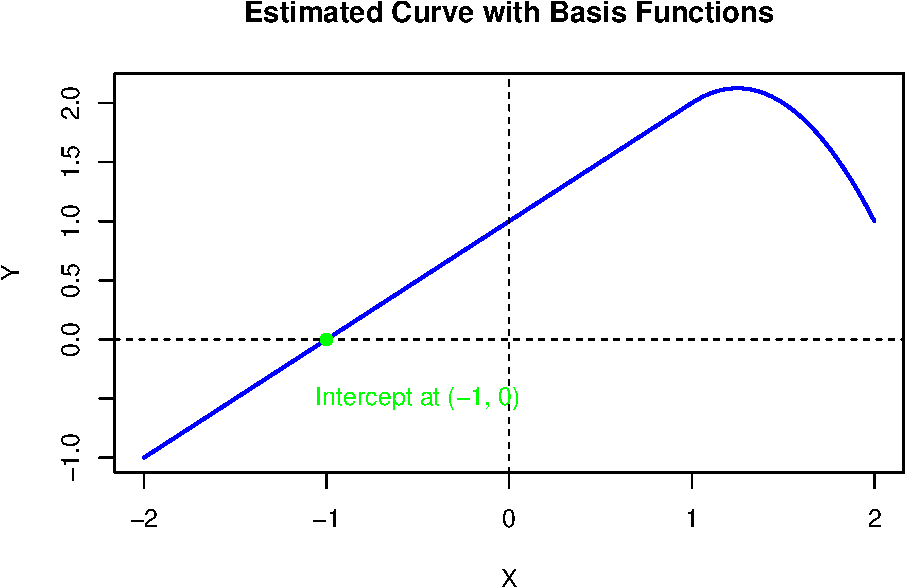
\includegraphics{chapter-07-hw_files/figure-latex/unnamed-chunk-1-1.pdf}

\begin{center}\rule{0.5\linewidth}{0.5pt}\end{center}

\subsection{Applied Questions}\label{applied-questions}

\paragraph{Exercise 6:}\label{exercise-6}

In this exercise, you will further analyze the \(\mathbf{Wage}\) data
set considered throughout this chapter.

\begin{enumerate}
\def\labelenumi{(\alph{enumi})}
\tightlist
\item
  Perform polynomial regression to predict wage using age. Use
  crossvalidation to select the optimal degree d for the polynomial.
  What degree was chosen, and how does this compare to the results of
  hypothesis testing using ANOVA? Make a plot of the resulting
  polynomial fit to the data.
\end{enumerate}

\begin{Shaded}
\begin{Highlighting}[]
\FunctionTok{data}\NormalTok{(Wage)}
\FunctionTok{set.seed}\NormalTok{(}\DecValTok{488}\NormalTok{)}

\CommentTok{\# cv for polynomial degrees 1–5}
\NormalTok{degrees }\OtherTok{\textless{}{-}} \DecValTok{1}\SpecialCharTok{:}\DecValTok{5}
\NormalTok{cv\_errors }\OtherTok{\textless{}{-}} \FunctionTok{numeric}\NormalTok{(}\FunctionTok{length}\NormalTok{(degrees))}

\ControlFlowTok{for}\NormalTok{ (d }\ControlFlowTok{in}\NormalTok{ degrees) \{}
  \CommentTok{\#  model formula with degree d}
\NormalTok{  model\_formula }\OtherTok{\textless{}{-}} \FunctionTok{as.formula}\NormalTok{(}\FunctionTok{paste}\NormalTok{(}\StringTok{"wage \textasciitilde{} poly(age,"}\NormalTok{, d, }\StringTok{")"}\NormalTok{))}
  
  \CommentTok{\#  10{-}fold cross{-}validation}
\NormalTok{  glm\_model }\OtherTok{\textless{}{-}} \FunctionTok{glm}\NormalTok{(model\_formula, }\AttributeTok{data =}\NormalTok{ Wage)}
\NormalTok{  cv\_results }\OtherTok{\textless{}{-}} \FunctionTok{cv.glm}\NormalTok{(Wage, glm\_model, }\AttributeTok{K =} \DecValTok{10}\NormalTok{)}
  
  \CommentTok{\# Store cross{-}validation error (MSE)}
\NormalTok{  cv\_errors[d] }\OtherTok{\textless{}{-}}\NormalTok{ cv\_results}\SpecialCharTok{$}\NormalTok{delta[}\DecValTok{1}\NormalTok{]}
\NormalTok{\}}

\CommentTok{\# Identify optimal degree with minimal CV error}
\NormalTok{optimal\_degree }\OtherTok{\textless{}{-}}\NormalTok{ degrees[}\FunctionTok{which.min}\NormalTok{(cv\_errors)]}
\FunctionTok{cat}\NormalTok{(}\StringTok{"Optimal polynomial degree from CV:"}\NormalTok{, optimal\_degree, }\StringTok{"}\SpecialCharTok{\textbackslash{}n}\StringTok{"}\NormalTok{)}
\end{Highlighting}
\end{Shaded}

\begin{verbatim}
## Optimal polynomial degree from CV: 4
\end{verbatim}

\begin{Shaded}
\begin{Highlighting}[]
\CommentTok{\# fit models for deg 1, ... ,4}
\NormalTok{fit\_1 }\OtherTok{\textless{}{-}} \FunctionTok{lm}\NormalTok{(wage }\SpecialCharTok{\textasciitilde{}} \FunctionTok{poly}\NormalTok{(age, }\DecValTok{1}\NormalTok{), }\AttributeTok{data =}\NormalTok{ Wage)  }
\NormalTok{fit\_2 }\OtherTok{\textless{}{-}} \FunctionTok{lm}\NormalTok{(wage }\SpecialCharTok{\textasciitilde{}} \FunctionTok{poly}\NormalTok{(age, }\DecValTok{2}\NormalTok{), }\AttributeTok{data =}\NormalTok{ Wage)  }
\NormalTok{fit\_3 }\OtherTok{\textless{}{-}} \FunctionTok{lm}\NormalTok{(wage }\SpecialCharTok{\textasciitilde{}} \FunctionTok{poly}\NormalTok{(age, }\DecValTok{3}\NormalTok{), }\AttributeTok{data =}\NormalTok{ Wage)  }
\NormalTok{fit\_4 }\OtherTok{\textless{}{-}} \FunctionTok{lm}\NormalTok{(wage }\SpecialCharTok{\textasciitilde{}} \FunctionTok{poly}\NormalTok{(age, }\DecValTok{4}\NormalTok{), }\AttributeTok{data =}\NormalTok{ Wage)  }

\CommentTok{\# comp models using ANOVA}
\NormalTok{anova\_results }\OtherTok{\textless{}{-}} \FunctionTok{anova}\NormalTok{(fit\_1, fit\_2, fit\_3, fit\_4)}
\FunctionTok{print}\NormalTok{(anova\_results)}
\end{Highlighting}
\end{Shaded}

\begin{verbatim}
## Analysis of Variance Table
## 
## Model 1: wage ~ poly(age, 1)
## Model 2: wage ~ poly(age, 2)
## Model 3: wage ~ poly(age, 3)
## Model 4: wage ~ poly(age, 4)
##   Res.Df     RSS Df Sum of Sq        F    Pr(>F)    
## 1   2998 5022216                                    
## 2   2997 4793430  1    228786 143.6025 < 2.2e-16 ***
## 3   2996 4777674  1     15756   9.8894  0.001679 ** 
## 4   2995 4771604  1      6070   3.8101  0.051039 .  
## ---
## Signif. codes:  0 '***' 0.001 '**' 0.01 '*' 0.05 '.' 0.1 ' ' 1
\end{verbatim}

From the output it would seem that cv of the polynomial regression tells
us that a 4th degree polynomial is the optimal choice. ANOVA analysis
however suggest that a 3rd degree is the best as it is the highest
degree that retains a p-value below 0.05.

\begin{enumerate}
\def\labelenumi{(\alph{enumi})}
\setcounter{enumi}{1}
\tightlist
\item
  Fit a step function to predict wage using age, and perform
  crossvalidation to choose the optimal number of cuts. Make a plot of
  the fit obtained.
\end{enumerate}

\begin{Shaded}
\begin{Highlighting}[]
\FunctionTok{set.seed}\NormalTok{(}\DecValTok{488}\NormalTok{)}
\NormalTok{K\_values }\OtherTok{\textless{}{-}} \DecValTok{2}\SpecialCharTok{:}\DecValTok{10}
\NormalTok{cv\_errors\_step }\OtherTok{\textless{}{-}} \FunctionTok{numeric}\NormalTok{(}\FunctionTok{length}\NormalTok{(K\_values))}

\CommentTok{\# age range from full dataset}
\NormalTok{age\_full }\OtherTok{\textless{}{-}}\NormalTok{ Wage}\SpecialCharTok{$}\NormalTok{age}
\NormalTok{min\_age }\OtherTok{\textless{}{-}} \FunctionTok{min}\NormalTok{(age\_full)}
\NormalTok{max\_age }\OtherTok{\textless{}{-}} \FunctionTok{max}\NormalTok{(age\_full)}

\ControlFlowTok{for}\NormalTok{ (k }\ControlFlowTok{in}\NormalTok{ K\_values) \{}
  \CommentTok{\# breaks based on dataset age range }
\NormalTok{  breaks }\OtherTok{\textless{}{-}} \FunctionTok{seq}\NormalTok{(min\_age, max\_age, }\AttributeTok{length.out =}\NormalTok{ k }\SpecialCharTok{+} \DecValTok{1}\NormalTok{)}
  
  \CommentTok{\# factor variable using breaks}
\NormalTok{  Wage}\SpecialCharTok{$}\NormalTok{age\_cut }\OtherTok{\textless{}{-}} \FunctionTok{cut}\NormalTok{(age\_full, }\AttributeTok{breaks =}\NormalTok{ breaks, }\AttributeTok{include.lowest =} \ConstantTok{TRUE}\NormalTok{)}
  
  \CommentTok{\# 10{-}X CV}
\NormalTok{  cv\_results }\OtherTok{\textless{}{-}} \FunctionTok{cv.glm}\NormalTok{(}
    \AttributeTok{data =}\NormalTok{ Wage,}
    \AttributeTok{glmfit =} \FunctionTok{glm}\NormalTok{(wage }\SpecialCharTok{\textasciitilde{}}\NormalTok{ age\_cut, }\AttributeTok{data =}\NormalTok{ Wage),}
    \AttributeTok{K =} \DecValTok{10}
\NormalTok{  )}
\NormalTok{  cv\_errors\_step[k }\SpecialCharTok{{-}} \DecValTok{1}\NormalTok{] }\OtherTok{\textless{}{-}}\NormalTok{ cv\_results}\SpecialCharTok{$}\NormalTok{delta[}\DecValTok{1}\NormalTok{]}
\NormalTok{\}}

\CommentTok{\# get optimal K}
\NormalTok{opt\_k }\OtherTok{\textless{}{-}}\NormalTok{ K\_values[}\FunctionTok{which.min}\NormalTok{(cv\_errors\_step)]}
\FunctionTok{cat}\NormalTok{(}\StringTok{"Optimal number of intervals from CV:"}\NormalTok{, opt\_k, }\StringTok{"}\SpecialCharTok{\textbackslash{}n}\StringTok{"}\NormalTok{)}
\end{Highlighting}
\end{Shaded}

\begin{verbatim}
## Optimal number of intervals from CV: 8
\end{verbatim}

\begin{Shaded}
\begin{Highlighting}[]
\CommentTok{\# fit model using opt k on full data}
\NormalTok{optimal\_breaks }\OtherTok{\textless{}{-}} \FunctionTok{seq}\NormalTok{(min\_age, max\_age, }\AttributeTok{length.out =}\NormalTok{ opt\_k }\SpecialCharTok{+} \DecValTok{1}\NormalTok{)}
\NormalTok{Wage}\SpecialCharTok{$}\NormalTok{age\_cut }\OtherTok{\textless{}{-}} \FunctionTok{cut}\NormalTok{(age\_full, }\AttributeTok{breaks =}\NormalTok{ optimal\_breaks, }\AttributeTok{include.lowest =} \ConstantTok{TRUE}\NormalTok{)}
\NormalTok{optimal\_step\_model }\OtherTok{\textless{}{-}} \FunctionTok{glm}\NormalTok{(wage }\SpecialCharTok{\textasciitilde{}}\NormalTok{ age\_cut, }\AttributeTok{data =}\NormalTok{ Wage)}

\CommentTok{\# get predictions for plot}
\NormalTok{pred\_data }\OtherTok{\textless{}{-}} \FunctionTok{data.frame}\NormalTok{(}\AttributeTok{age =} \FunctionTok{seq}\NormalTok{(min\_age, max\_age, }\AttributeTok{length.out =} \DecValTok{1000}\NormalTok{))}
\NormalTok{pred\_data}\SpecialCharTok{$}\NormalTok{age\_cut }\OtherTok{\textless{}{-}} \FunctionTok{cut}\NormalTok{(pred\_data}\SpecialCharTok{$}\NormalTok{age, }\AttributeTok{breaks =}\NormalTok{ optimal\_breaks, }\AttributeTok{include.lowest =} \ConstantTok{TRUE}\NormalTok{)}
\NormalTok{pred\_data}\SpecialCharTok{$}\NormalTok{wage\_pred }\OtherTok{\textless{}{-}} \FunctionTok{predict}\NormalTok{(optimal\_step\_model, }\AttributeTok{newdata =}\NormalTok{ pred\_data)}

\CommentTok{\# plot step func fit}
\FunctionTok{ggplot}\NormalTok{(Wage, }\FunctionTok{aes}\NormalTok{(}\AttributeTok{x =}\NormalTok{ age, }\AttributeTok{y =}\NormalTok{ wage)) }\SpecialCharTok{+}
  \FunctionTok{geom\_point}\NormalTok{(}\AttributeTok{alpha =} \FloatTok{0.2}\NormalTok{, }\AttributeTok{color =} \StringTok{"gray50"}\NormalTok{) }\SpecialCharTok{+}
  \FunctionTok{geom\_step}\NormalTok{(}
    \AttributeTok{data =}\NormalTok{ pred\_data,}
    \FunctionTok{aes}\NormalTok{(}\AttributeTok{x =}\NormalTok{ age, }\AttributeTok{y =}\NormalTok{ wage\_pred),}
    \AttributeTok{color =} \StringTok{"red"}\NormalTok{,}
    \AttributeTok{linewidth =} \DecValTok{1}
\NormalTok{  ) }\SpecialCharTok{+}
  \FunctionTok{labs}\NormalTok{(}
    \AttributeTok{title =} \FunctionTok{paste}\NormalTok{(}\StringTok{"Step Function Fit with"}\NormalTok{, opt\_k, }\StringTok{"Intervals"}\NormalTok{),}
    \AttributeTok{x =} \StringTok{"Age"}\NormalTok{,}
    \AttributeTok{y =} \StringTok{"Wage"}
\NormalTok{  ) }\SpecialCharTok{+}
  \FunctionTok{theme\_minimal}\NormalTok{()}
\end{Highlighting}
\end{Shaded}

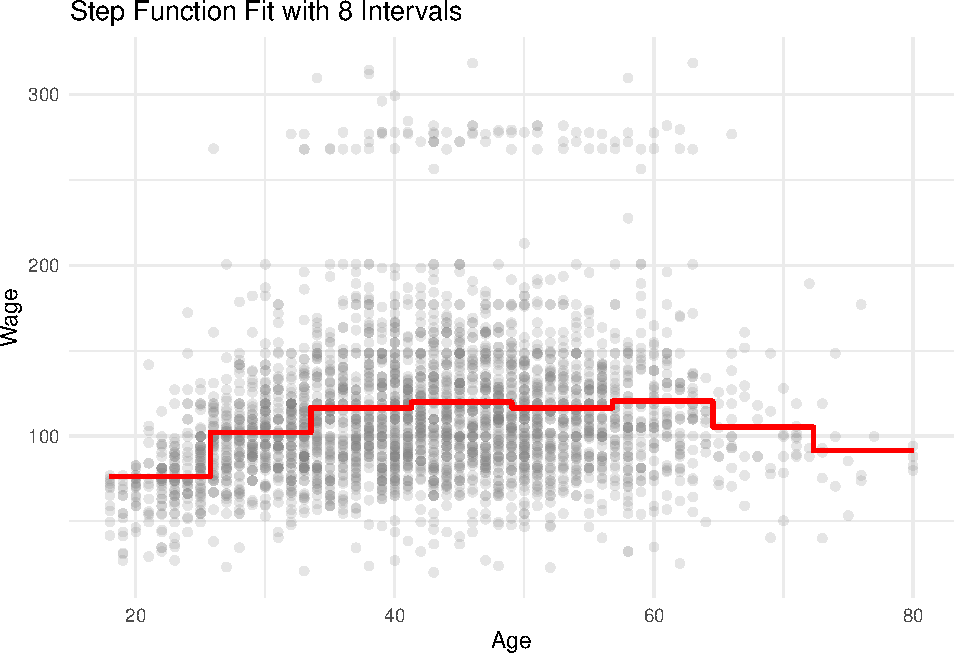
\includegraphics{chapter-07-hw_files/figure-latex/unnamed-chunk-3-1.pdf}

\paragraph{Exercise 9:}\label{exercise-9}

This question uses the variables dis (the weighted mean of distances to
five Boston employment centers) and nox (nitrogen oxides concentration
in parts per 10 million) from the Boston data. We will treat dis as the
predictor and nox as the response.

\begin{enumerate}
\def\labelenumi{(\alph{enumi})}
\tightlist
\item
  Use the poly() function to fit a cubic polynomial regression to
  predict nox using dis. Report the regression output, and plot the
  resulting data and polynomial fits.
\end{enumerate}

\begin{Shaded}
\begin{Highlighting}[]
\FunctionTok{data}\NormalTok{(Boston)}
\FunctionTok{set.seed}\NormalTok{(}\DecValTok{488}\NormalTok{)}
\CommentTok{\# cubic poly regression}
\NormalTok{cubic\_model }\OtherTok{\textless{}{-}} \FunctionTok{lm}\NormalTok{(nox }\SpecialCharTok{\textasciitilde{}} \FunctionTok{poly}\NormalTok{(dis, }\DecValTok{3}\NormalTok{), }\AttributeTok{data =}\NormalTok{ Boston)}
\FunctionTok{summary}\NormalTok{(cubic\_model)}
\end{Highlighting}
\end{Shaded}

\begin{verbatim}
## 
## Call:
## lm(formula = nox ~ poly(dis, 3), data = Boston)
## 
## Residuals:
##       Min        1Q    Median        3Q       Max 
## -0.121130 -0.040619 -0.009738  0.023385  0.194904 
## 
## Coefficients:
##                Estimate Std. Error t value Pr(>|t|)    
## (Intercept)    0.554695   0.002759 201.021  < 2e-16 ***
## poly(dis, 3)1 -2.003096   0.062071 -32.271  < 2e-16 ***
## poly(dis, 3)2  0.856330   0.062071  13.796  < 2e-16 ***
## poly(dis, 3)3 -0.318049   0.062071  -5.124 4.27e-07 ***
## ---
## Signif. codes:  0 '***' 0.001 '**' 0.01 '*' 0.05 '.' 0.1 ' ' 1
## 
## Residual standard error: 0.06207 on 502 degrees of freedom
## Multiple R-squared:  0.7148, Adjusted R-squared:  0.7131 
## F-statistic: 419.3 on 3 and 502 DF,  p-value: < 2.2e-16
\end{verbatim}

\begin{Shaded}
\begin{Highlighting}[]
\CommentTok{\# predictions for plot}
\NormalTok{pred\_data }\OtherTok{\textless{}{-}} \FunctionTok{data.frame}\NormalTok{(}\AttributeTok{dis =} \FunctionTok{seq}\NormalTok{(}\FunctionTok{min}\NormalTok{(Boston}\SpecialCharTok{$}\NormalTok{dis), }\FunctionTok{max}\NormalTok{(Boston}\SpecialCharTok{$}\NormalTok{dis), }\AttributeTok{length.out =} \DecValTok{100}\NormalTok{))}
\NormalTok{pred\_data}\SpecialCharTok{$}\NormalTok{nox\_pred }\OtherTok{\textless{}{-}} \FunctionTok{predict}\NormalTok{(cubic\_model, }\AttributeTok{newdata =}\NormalTok{ pred\_data)}
\CommentTok{\# plot data , polynomial fit}
\FunctionTok{ggplot}\NormalTok{(Boston, }\FunctionTok{aes}\NormalTok{(}\AttributeTok{x =}\NormalTok{ dis, }\AttributeTok{y =}\NormalTok{ nox)) }\SpecialCharTok{+}
  \FunctionTok{geom\_point}\NormalTok{(}\AttributeTok{alpha =} \FloatTok{0.2}\NormalTok{, }\AttributeTok{color =} \StringTok{"gray50"}\NormalTok{) }\SpecialCharTok{+}
  \FunctionTok{geom\_line}\NormalTok{(}\AttributeTok{data =}\NormalTok{ pred\_data, }\FunctionTok{aes}\NormalTok{(}\AttributeTok{x =}\NormalTok{ dis, }\AttributeTok{y =}\NormalTok{ nox\_pred), }\AttributeTok{color =} \StringTok{"blue"}\NormalTok{, }\AttributeTok{linewidth =} \DecValTok{1}\NormalTok{) }\SpecialCharTok{+}
  \FunctionTok{labs}\NormalTok{(}\AttributeTok{title =} \StringTok{"Cubic Polynomial Fit to Predict NOx using DIS"}\NormalTok{,}
       \AttributeTok{x =} \StringTok{"DIS (Distance to Employment Centers)"}\NormalTok{,}
       \AttributeTok{y =} \StringTok{"NOx (Nitrogen Oxides Concentration)"}\NormalTok{) }\SpecialCharTok{+}
  \FunctionTok{theme\_minimal}\NormalTok{()}
\end{Highlighting}
\end{Shaded}

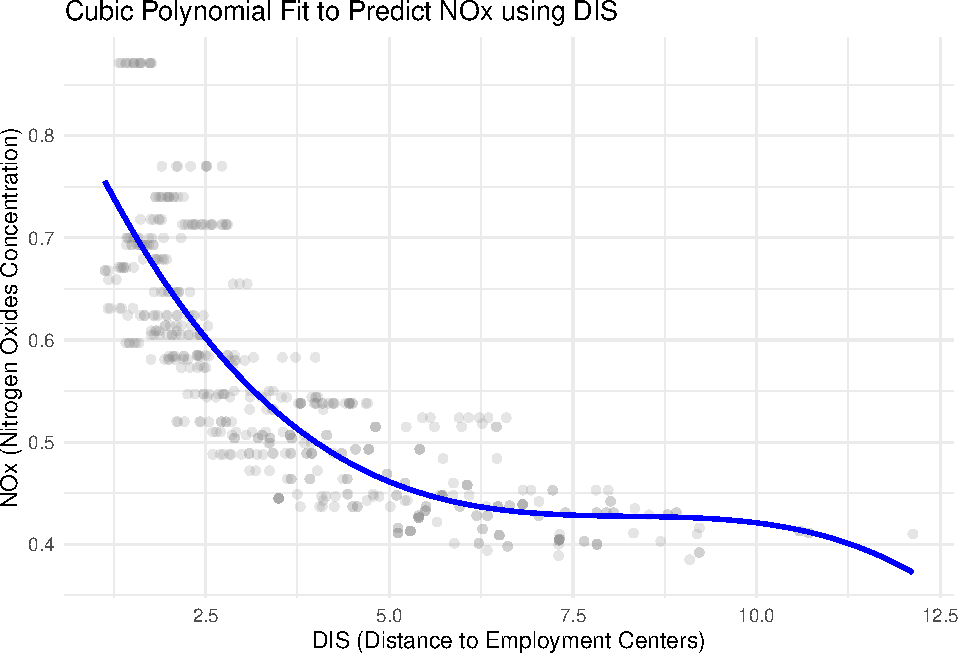
\includegraphics{chapter-07-hw_files/figure-latex/unnamed-chunk-4-1.pdf}

\begin{enumerate}
\def\labelenumi{(\alph{enumi})}
\setcounter{enumi}{1}
\tightlist
\item
  Plot the polynomial fits for a range of different polynomial degrees
  (say, from 1 to 10), and report the associated residual sum of
  squares.
\end{enumerate}

\begin{Shaded}
\begin{Highlighting}[]
\CommentTok{\# polynomial regression for degrees 1 to 10}
\NormalTok{degrees\_poly }\OtherTok{\textless{}{-}} \DecValTok{1}\SpecialCharTok{:}\DecValTok{10}
\NormalTok{rss\_poly }\OtherTok{\textless{}{-}} \FunctionTok{numeric}\NormalTok{(}\FunctionTok{length}\NormalTok{(degrees\_poly))}
\ControlFlowTok{for}\NormalTok{ (d }\ControlFlowTok{in}\NormalTok{ degrees\_poly) \{}
  \CommentTok{\# fit polynomial model}
\NormalTok{  poly\_model }\OtherTok{\textless{}{-}} \FunctionTok{lm}\NormalTok{(nox }\SpecialCharTok{\textasciitilde{}} \FunctionTok{poly}\NormalTok{(dis, d), }\AttributeTok{data =}\NormalTok{ Boston)}
  
  \CommentTok{\# rss}
\NormalTok{  rss\_poly[d] }\OtherTok{\textless{}{-}} \FunctionTok{sum}\NormalTok{(}\FunctionTok{residuals}\NormalTok{(poly\_model)}\SpecialCharTok{\^{}}\DecValTok{2}\NormalTok{)}
\NormalTok{\}}
\CommentTok{\#  RSS for different polynomial degrees}
\NormalTok{rss\_data }\OtherTok{\textless{}{-}} \FunctionTok{data.frame}\NormalTok{(}\AttributeTok{Degree =}\NormalTok{ degrees\_poly, }\AttributeTok{RSS =}\NormalTok{ rss\_poly)}
\FunctionTok{ggplot}\NormalTok{(rss\_data, }\FunctionTok{aes}\NormalTok{(}\AttributeTok{x =}\NormalTok{ Degree, }\AttributeTok{y =}\NormalTok{ RSS)) }\SpecialCharTok{+}
  \FunctionTok{geom\_line}\NormalTok{(}\AttributeTok{color =} \StringTok{"red"}\NormalTok{, }\AttributeTok{size =} \DecValTok{1}\NormalTok{) }\SpecialCharTok{+}
  \FunctionTok{geom\_point}\NormalTok{(}\AttributeTok{size =} \DecValTok{3}\NormalTok{) }\SpecialCharTok{+}
  \FunctionTok{labs}\NormalTok{(}\AttributeTok{title =} \StringTok{"Residual Sum of Squares for Polynomial Degrees"}\NormalTok{,}
       \AttributeTok{x =} \StringTok{"Polynomial Degree"}\NormalTok{,}
       \AttributeTok{y =} \StringTok{"Residual Sum of Squares (RSS)"}\NormalTok{) }\SpecialCharTok{+}
  \FunctionTok{theme\_minimal}\NormalTok{()}
\end{Highlighting}
\end{Shaded}

\begin{verbatim}
## Warning: Using `size` aesthetic for lines was deprecated in ggplot2 3.4.0.
## i Please use `linewidth` instead.
## This warning is displayed once every 8 hours.
## Call `lifecycle::last_lifecycle_warnings()` to see where this warning was
## generated.
\end{verbatim}

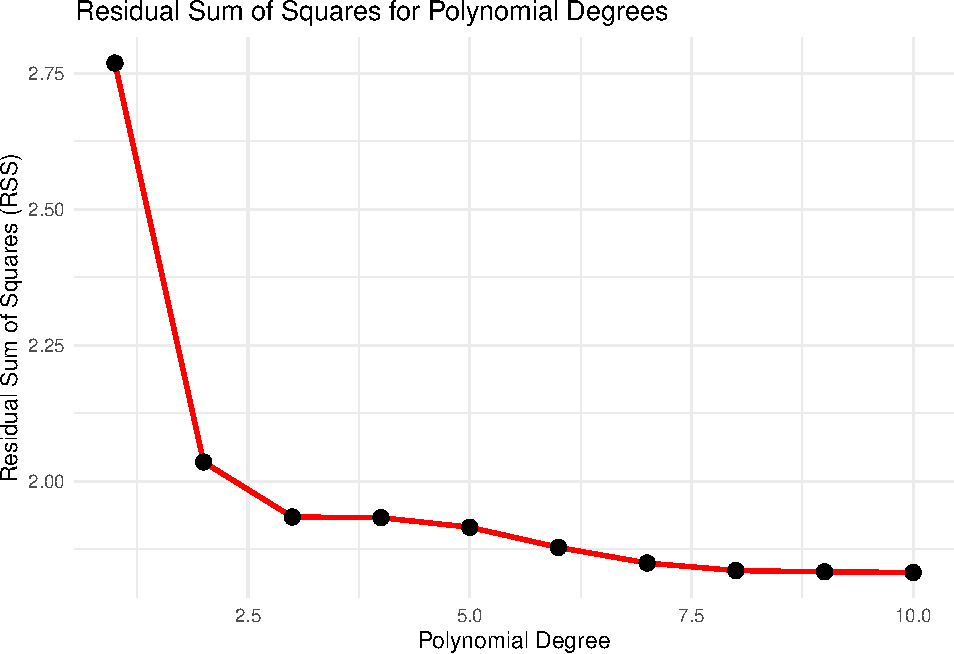
\includegraphics{chapter-07-hw_files/figure-latex/unnamed-chunk-5-1.pdf}

\begin{Shaded}
\begin{Highlighting}[]
\CommentTok{\# RSS values}
\FunctionTok{print}\NormalTok{(rss\_data)}
\end{Highlighting}
\end{Shaded}

\begin{verbatim}
##    Degree      RSS
## 1       1 2.768563
## 2       2 2.035262
## 3       3 1.934107
## 4       4 1.932981
## 5       5 1.915290
## 6       6 1.878257
## 7       7 1.849484
## 8       8 1.835630
## 9       9 1.833331
## 10     10 1.832171
\end{verbatim}

\begin{Shaded}
\begin{Highlighting}[]
\CommentTok{\# RSS values for each degree}
\ControlFlowTok{for}\NormalTok{ (i }\ControlFlowTok{in} \DecValTok{1}\SpecialCharTok{:}\FunctionTok{length}\NormalTok{(degrees\_poly)) \{}
  \FunctionTok{cat}\NormalTok{(}\StringTok{"Degree"}\NormalTok{, degrees\_poly[i], }\StringTok{"RSS:"}\NormalTok{, rss\_poly[i], }\StringTok{"}\SpecialCharTok{\textbackslash{}n}\StringTok{"}\NormalTok{)}
\NormalTok{\}}
\end{Highlighting}
\end{Shaded}

\begin{verbatim}
## Degree 1 RSS: 2.768563 
## Degree 2 RSS: 2.035262 
## Degree 3 RSS: 1.934107 
## Degree 4 RSS: 1.932981 
## Degree 5 RSS: 1.91529 
## Degree 6 RSS: 1.878257 
## Degree 7 RSS: 1.849484 
## Degree 8 RSS: 1.83563 
## Degree 9 RSS: 1.833331 
## Degree 10 RSS: 1.832171
\end{verbatim}

\begin{enumerate}
\def\labelenumi{(\alph{enumi})}
\setcounter{enumi}{2}
\tightlist
\item
  Perform cross-validation or another approach to select the optimal
  degree for the polynomial, and explain your results.
\end{enumerate}

\begin{Shaded}
\begin{Highlighting}[]
\FunctionTok{set.seed}\NormalTok{(}\DecValTok{488}\NormalTok{)}
\NormalTok{degrees\_poly }\OtherTok{\textless{}{-}} \DecValTok{1}\SpecialCharTok{:}\DecValTok{10}
\NormalTok{cv\_errors\_poly }\OtherTok{\textless{}{-}} \FunctionTok{numeric}\NormalTok{(}\FunctionTok{length}\NormalTok{(degrees\_poly))}

\ControlFlowTok{for}\NormalTok{ (d }\ControlFlowTok{in}\NormalTok{ degrees\_poly) \{}
\NormalTok{  model\_formula }\OtherTok{\textless{}{-}} \FunctionTok{as.formula}\NormalTok{(}\FunctionTok{paste}\NormalTok{(}\StringTok{"nox \textasciitilde{} poly(dis,"}\NormalTok{, d, }\StringTok{")"}\NormalTok{))}
  
  \CommentTok{\# GLM and perform 10{-}X CV}
\NormalTok{  glm\_model }\OtherTok{\textless{}{-}} \FunctionTok{glm}\NormalTok{(model\_formula, }\AttributeTok{data =}\NormalTok{ Boston)}
\NormalTok{  cv\_results }\OtherTok{\textless{}{-}} \FunctionTok{cv.glm}\NormalTok{(Boston, glm\_model, }\AttributeTok{K =} \DecValTok{10}\NormalTok{)}
  
  \CommentTok{\#  CV error }
\NormalTok{  cv\_errors\_poly[d] }\OtherTok{\textless{}{-}}\NormalTok{ cv\_results}\SpecialCharTok{$}\NormalTok{delta[}\DecValTok{1}\NormalTok{]}
\NormalTok{\}}

\CommentTok{\# optimal degree}
\NormalTok{opt\_poly }\OtherTok{\textless{}{-}}\NormalTok{ degrees\_poly[}\FunctionTok{which.min}\NormalTok{(cv\_errors\_poly)]}
\FunctionTok{cat}\NormalTok{(}\StringTok{"Optimal polynomial degree from CV:"}\NormalTok{, opt\_poly, }\StringTok{"}\SpecialCharTok{\textbackslash{}n}\StringTok{"}\NormalTok{)}
\end{Highlighting}
\end{Shaded}

\begin{verbatim}
## Optimal polynomial degree from CV: 3
\end{verbatim}

\begin{Shaded}
\begin{Highlighting}[]
\CommentTok{\# CV errors}
\FunctionTok{ggplot}\NormalTok{(}\FunctionTok{data.frame}\NormalTok{(}\AttributeTok{Degree =}\NormalTok{ degrees\_poly, }\AttributeTok{CV\_Error =}\NormalTok{ cv\_errors\_poly), }
       \FunctionTok{aes}\NormalTok{(}\AttributeTok{x =}\NormalTok{ Degree, }\AttributeTok{y =}\NormalTok{ CV\_Error)) }\SpecialCharTok{+}
  \FunctionTok{geom\_line}\NormalTok{(}\AttributeTok{color =} \StringTok{"blue"}\NormalTok{, }\AttributeTok{linewidth =} \DecValTok{1}\NormalTok{) }\SpecialCharTok{+}
  \FunctionTok{geom\_point}\NormalTok{(}\AttributeTok{size =} \DecValTok{3}\NormalTok{) }\SpecialCharTok{+}
  \FunctionTok{labs}\NormalTok{(}\AttributeTok{title =} \StringTok{"Cross{-}Validation Error by Polynomial Degree"}\NormalTok{,}
       \AttributeTok{x =} \StringTok{"Degree"}\NormalTok{,}
       \AttributeTok{y =} \StringTok{"CV MSE"}\NormalTok{) }\SpecialCharTok{+}
  \FunctionTok{theme\_minimal}\NormalTok{()}
\end{Highlighting}
\end{Shaded}

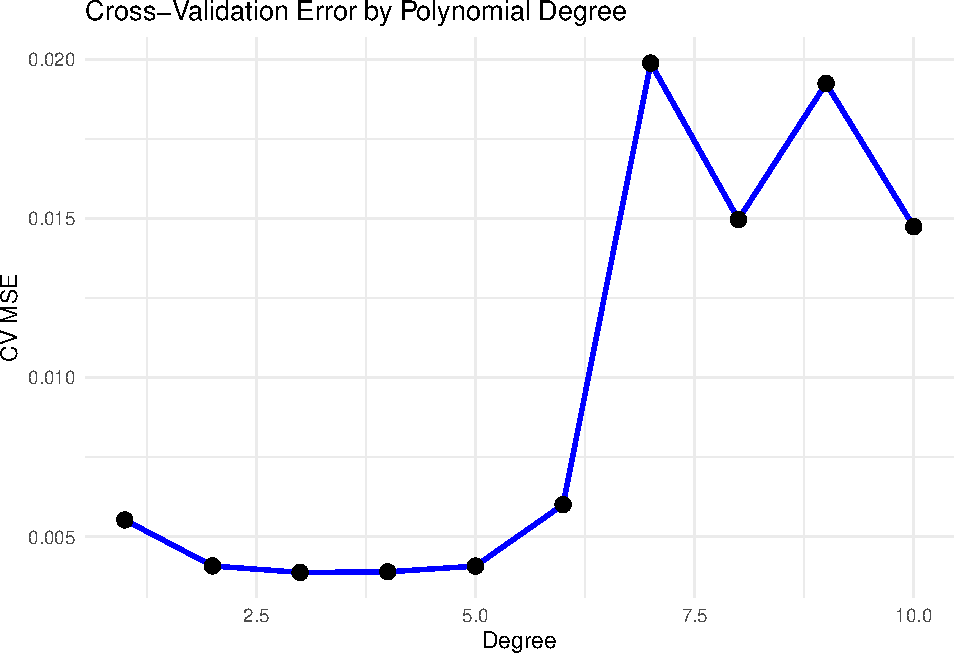
\includegraphics{chapter-07-hw_files/figure-latex/unnamed-chunk-6-1.pdf}
From the result of the cross-validation, degree 3 balances bias and
variance, yielding the lowest mean CV error, so it is the best selection
over higher‑degree polynomials which may have extra flexibility however
this doesnt necessarily mean they will result in a better prediction.

\begin{enumerate}
\def\labelenumi{(\alph{enumi})}
\setcounter{enumi}{3}
\tightlist
\item
  Use the bs() function to fit a regression spline to predict nox using
  dis. Report the output for the fit using four degrees of freedom. How
  did you choose the knots? Plot the resulting fit.
\end{enumerate}

\begin{Shaded}
\begin{Highlighting}[]
\CommentTok{\# spline with df=4 }
\NormalTok{spline\_4df }\OtherTok{\textless{}{-}} \FunctionTok{lm}\NormalTok{(nox }\SpecialCharTok{\textasciitilde{}} \FunctionTok{bs}\NormalTok{(dis, }\AttributeTok{df =} \DecValTok{4}\NormalTok{), }\AttributeTok{data =}\NormalTok{ Boston)}

\CommentTok{\# knots \& model summary}
\NormalTok{knots\_4df }\OtherTok{\textless{}{-}} \FunctionTok{attr}\NormalTok{(}\FunctionTok{bs}\NormalTok{(Boston}\SpecialCharTok{$}\NormalTok{dis, }\AttributeTok{df =} \DecValTok{4}\NormalTok{), }\StringTok{"knots"}\NormalTok{)}
\FunctionTok{cat}\NormalTok{(}\StringTok{"Knot locations for df=4:"}\NormalTok{, knots\_4df, }\StringTok{"}\SpecialCharTok{\textbackslash{}n}\StringTok{"}\NormalTok{)}
\end{Highlighting}
\end{Shaded}

\begin{verbatim}
## Knot locations for df=4: 3.20745
\end{verbatim}

\begin{Shaded}
\begin{Highlighting}[]
\FunctionTok{summary}\NormalTok{(spline\_4df)}
\end{Highlighting}
\end{Shaded}

\begin{verbatim}
## 
## Call:
## lm(formula = nox ~ bs(dis, df = 4), data = Boston)
## 
## Residuals:
##       Min        1Q    Median        3Q       Max 
## -0.124622 -0.039259 -0.008514  0.020850  0.193891 
## 
## Coefficients:
##                  Estimate Std. Error t value Pr(>|t|)    
## (Intercept)       0.73447    0.01460  50.306  < 2e-16 ***
## bs(dis, df = 4)1 -0.05810    0.02186  -2.658  0.00812 ** 
## bs(dis, df = 4)2 -0.46356    0.02366 -19.596  < 2e-16 ***
## bs(dis, df = 4)3 -0.19979    0.04311  -4.634 4.58e-06 ***
## bs(dis, df = 4)4 -0.38881    0.04551  -8.544  < 2e-16 ***
## ---
## Signif. codes:  0 '***' 0.001 '**' 0.01 '*' 0.05 '.' 0.1 ' ' 1
## 
## Residual standard error: 0.06195 on 501 degrees of freedom
## Multiple R-squared:  0.7164, Adjusted R-squared:  0.7142 
## F-statistic: 316.5 on 4 and 501 DF,  p-value: < 2.2e-16
\end{verbatim}

\begin{Shaded}
\begin{Highlighting}[]
\CommentTok{\# spline fit}
\NormalTok{pred\_data }\OtherTok{\textless{}{-}} \FunctionTok{data.frame}\NormalTok{(}\AttributeTok{dis =} \FunctionTok{seq}\NormalTok{(}\FunctionTok{min}\NormalTok{(Boston}\SpecialCharTok{$}\NormalTok{dis), }\FunctionTok{max}\NormalTok{(Boston}\SpecialCharTok{$}\NormalTok{dis), }\AttributeTok{length.out =} \DecValTok{100}\NormalTok{))}
\NormalTok{pred\_data}\SpecialCharTok{$}\NormalTok{nox\_pred }\OtherTok{\textless{}{-}} \FunctionTok{predict}\NormalTok{(spline\_4df, }\AttributeTok{newdata =}\NormalTok{ pred\_data)}

\FunctionTok{ggplot}\NormalTok{(Boston, }\FunctionTok{aes}\NormalTok{(}\AttributeTok{x =}\NormalTok{ dis, }\AttributeTok{y =}\NormalTok{ nox)) }\SpecialCharTok{+}
  \FunctionTok{geom\_point}\NormalTok{(}\AttributeTok{alpha =} \FloatTok{0.2}\NormalTok{, }\AttributeTok{color =} \StringTok{"gray50"}\NormalTok{) }\SpecialCharTok{+}
  \FunctionTok{geom\_line}\NormalTok{(}\AttributeTok{data =}\NormalTok{ pred\_data, }\FunctionTok{aes}\NormalTok{(}\AttributeTok{x =}\NormalTok{ dis, }\AttributeTok{y =}\NormalTok{ nox\_pred), }\AttributeTok{color =} \StringTok{"green"}\NormalTok{, }\AttributeTok{linewidth =} \DecValTok{1}\NormalTok{) }\SpecialCharTok{+}
  \FunctionTok{labs}\NormalTok{(}\AttributeTok{title =} \StringTok{"Regression Spline Fit (df=4)"}\NormalTok{,}
       \AttributeTok{x =} \StringTok{"DIS"}\NormalTok{,}
       \AttributeTok{y =} \StringTok{"NOx"}\NormalTok{) }\SpecialCharTok{+}
  \FunctionTok{theme\_minimal}\NormalTok{()}
\end{Highlighting}
\end{Shaded}

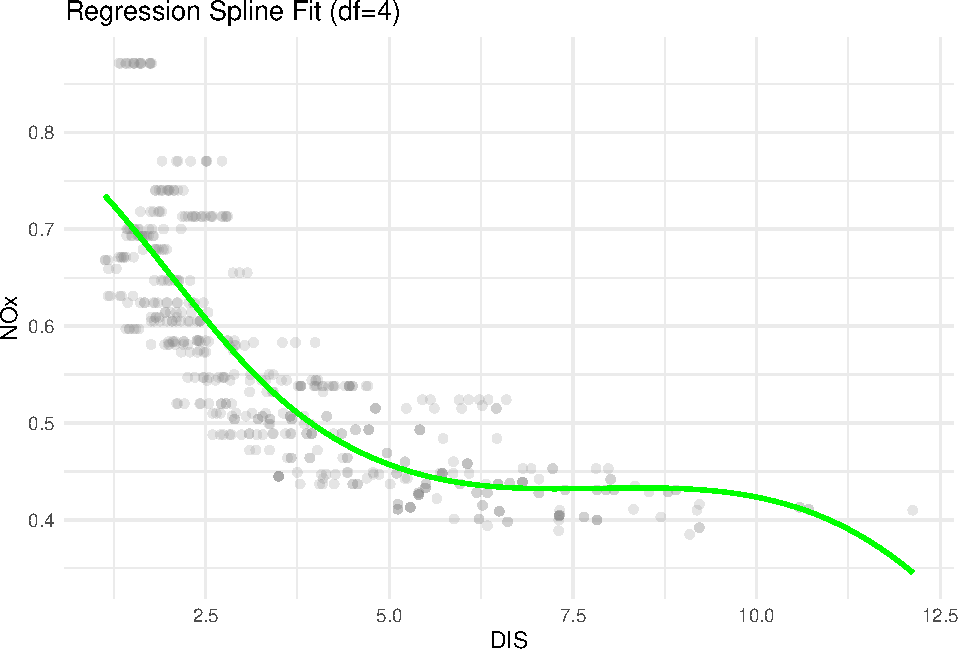
\includegraphics{chapter-07-hw_files/figure-latex/unnamed-chunk-7-1.pdf}
The placement of knots is determined by the data distribution and the
number of degrees of freedom. In this case, we used 4 degrees of
freedom, which allows for a flexible fit while avoiding overfitting. The
knots are placed at quantiles of the predictor variable by default this
may help the spline better convey the underlying structure in the data.

\begin{enumerate}
\def\labelenumi{(\alph{enumi})}
\setcounter{enumi}{4}
\tightlist
\item
  Now fit a regression spline for a range of degrees of freedom, and
  plot the resulting fits and report the resulting RSS. Describe the
  results obtained.
\end{enumerate}

\begin{Shaded}
\begin{Highlighting}[]
\NormalTok{df\_values }\OtherTok{\textless{}{-}} \DecValTok{3}\SpecialCharTok{:}\DecValTok{10}
\NormalTok{rss\_spline }\OtherTok{\textless{}{-}} \FunctionTok{numeric}\NormalTok{(}\FunctionTok{length}\NormalTok{(df\_values))}

\ControlFlowTok{for}\NormalTok{ (i }\ControlFlowTok{in} \FunctionTok{seq\_along}\NormalTok{(df\_values)) \{}
\NormalTok{  spline\_model }\OtherTok{\textless{}{-}} \FunctionTok{lm}\NormalTok{(nox }\SpecialCharTok{\textasciitilde{}} \FunctionTok{bs}\NormalTok{(dis, }\AttributeTok{df =}\NormalTok{ df\_values[i]), }\AttributeTok{data =}\NormalTok{ Boston)}
\NormalTok{  rss\_spline[i] }\OtherTok{\textless{}{-}} \FunctionTok{sum}\NormalTok{(}\FunctionTok{residuals}\NormalTok{(spline\_model)}\SpecialCharTok{\^{}}\DecValTok{2}\NormalTok{)}
\NormalTok{\}}

\CommentTok{\# RSS vs df}
\FunctionTok{ggplot}\NormalTok{(}\FunctionTok{data.frame}\NormalTok{(}\AttributeTok{DF =}\NormalTok{ df\_values, }\AttributeTok{RSS =}\NormalTok{ rss\_spline), }\FunctionTok{aes}\NormalTok{(}\AttributeTok{x =}\NormalTok{ DF, }\AttributeTok{y =}\NormalTok{ RSS)) }\SpecialCharTok{+}
  \FunctionTok{geom\_line}\NormalTok{(}\AttributeTok{color =} \StringTok{"purple"}\NormalTok{, }\AttributeTok{linewidth =} \DecValTok{1}\NormalTok{) }\SpecialCharTok{+}
  \FunctionTok{geom\_point}\NormalTok{(}\AttributeTok{size =} \DecValTok{3}\NormalTok{) }\SpecialCharTok{+}
  \FunctionTok{labs}\NormalTok{(}\AttributeTok{title =} \StringTok{"RSS for Regression Splines"}\NormalTok{,}
       \AttributeTok{x =} \StringTok{"Degrees of Freedom"}\NormalTok{,}
       \AttributeTok{y =} \StringTok{"Residual Sum of Squares"}\NormalTok{) }\SpecialCharTok{+}
  \FunctionTok{theme\_minimal}\NormalTok{()}
\end{Highlighting}
\end{Shaded}

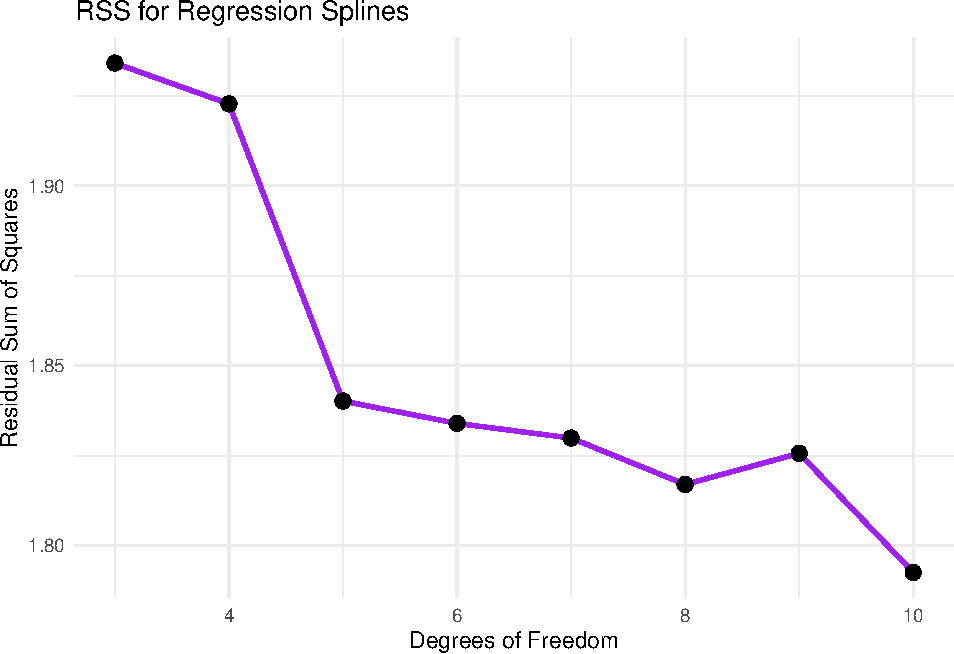
\includegraphics{chapter-07-hw_files/figure-latex/unnamed-chunk-8-1.pdf}

\begin{Shaded}
\begin{Highlighting}[]
\CommentTok{\# RSS values}
\FunctionTok{cat}\NormalTok{(}\StringTok{"RSS for Splines:}\SpecialCharTok{\textbackslash{}n}\StringTok{"}\NormalTok{)}
\end{Highlighting}
\end{Shaded}

\begin{verbatim}
## RSS for Splines:
\end{verbatim}

\begin{Shaded}
\begin{Highlighting}[]
\FunctionTok{print}\NormalTok{(}\FunctionTok{data.frame}\NormalTok{(}\AttributeTok{DF =}\NormalTok{ df\_values, }\AttributeTok{RSS =}\NormalTok{ rss\_spline))}
\end{Highlighting}
\end{Shaded}

\begin{verbatim}
##   DF      RSS
## 1  3 1.934107
## 2  4 1.922775
## 3  5 1.840173
## 4  6 1.833966
## 5  7 1.829884
## 6  8 1.816995
## 7  9 1.825653
## 8 10 1.792535
\end{verbatim}

The RSS values indicate that as the degrees of freedom increase, the RSS
tends to decrease, suggesting a better fit to the training data.
However, this levels off, suggesting that additional knots beyond
\(\approx 6\) capture little extra signal and mostly fit noise. The
optimal degree of freedom should balance bias and variance.

\begin{enumerate}
\def\labelenumi{(\alph{enumi})}
\setcounter{enumi}{5}
\tightlist
\item
  Perform cross-validation or another approach in order to select the
  best degrees of freedom for a regression spline on this data. Describe
  your results.
\end{enumerate}

\begin{Shaded}
\begin{Highlighting}[]
\FunctionTok{set.seed}\NormalTok{(}\DecValTok{488}\NormalTok{)}
\NormalTok{cv\_errors\_spline }\OtherTok{\textless{}{-}} \FunctionTok{numeric}\NormalTok{(}\FunctionTok{length}\NormalTok{(df\_values))}

\ControlFlowTok{for}\NormalTok{ (i }\ControlFlowTok{in} \FunctionTok{seq\_along}\NormalTok{(df\_values)) \{}
  \CommentTok{\# model formula}
\NormalTok{  model\_formula }\OtherTok{\textless{}{-}} \FunctionTok{as.formula}\NormalTok{(}\FunctionTok{paste}\NormalTok{(}\StringTok{"nox \textasciitilde{} bs(dis, df ="}\NormalTok{, df\_values[i], }\StringTok{")"}\NormalTok{))}
  
  \CommentTok{\# fit GLM , perform 10{-}X CV}
\NormalTok{  glm\_model }\OtherTok{\textless{}{-}} \FunctionTok{glm}\NormalTok{(model\_formula, }\AttributeTok{data =}\NormalTok{ Boston)}
\NormalTok{  cv\_results }\OtherTok{\textless{}{-}} \FunctionTok{cv.glm}\NormalTok{(Boston, glm\_model, }\AttributeTok{K =} \DecValTok{10}\NormalTok{)}
  
  \CommentTok{\# CV error}
\NormalTok{  cv\_errors\_spline[i] }\OtherTok{\textless{}{-}}\NormalTok{ cv\_results}\SpecialCharTok{$}\NormalTok{delta[}\DecValTok{1}\NormalTok{]}
\NormalTok{\}}
\end{Highlighting}
\end{Shaded}

\begin{verbatim}
## Warning in bs(dis, degree = 3L, knots = numeric(0), Boundary.knots = c(1.137, :
## some 'x' values beyond boundary knots may cause ill-conditioned bases
## Warning in bs(dis, degree = 3L, knots = numeric(0), Boundary.knots = c(1.137, :
## some 'x' values beyond boundary knots may cause ill-conditioned bases
\end{verbatim}

\begin{verbatim}
## Warning in bs(dis, degree = 3L, knots = numeric(0), Boundary.knots = c(1.1296,
## : some 'x' values beyond boundary knots may cause ill-conditioned bases
## Warning in bs(dis, degree = 3L, knots = numeric(0), Boundary.knots = c(1.1296,
## : some 'x' values beyond boundary knots may cause ill-conditioned bases
\end{verbatim}

\begin{verbatim}
## Warning in bs(dis, degree = 3L, knots = c(`50%` = 3.2157), Boundary.knots =
## c(1.1296, : some 'x' values beyond boundary knots may cause ill-conditioned
## bases
## Warning in bs(dis, degree = 3L, knots = c(`50%` = 3.2157), Boundary.knots =
## c(1.1296, : some 'x' values beyond boundary knots may cause ill-conditioned
## bases
\end{verbatim}

\begin{verbatim}
## Warning in bs(dis, degree = 3L, knots = c(`50%` = 3.1222), Boundary.knots =
## c(1.137, : some 'x' values beyond boundary knots may cause ill-conditioned
## bases
## Warning in bs(dis, degree = 3L, knots = c(`50%` = 3.1222), Boundary.knots =
## c(1.137, : some 'x' values beyond boundary knots may cause ill-conditioned
## bases
\end{verbatim}

\begin{verbatim}
## Warning in bs(dis, degree = 3L, knots = c(`33.33333%` = 2.3546, `66.66667%` =
## 4.23906666666667: some 'x' values beyond boundary knots may cause
## ill-conditioned bases
## Warning in bs(dis, degree = 3L, knots = c(`33.33333%` = 2.3546, `66.66667%` =
## 4.23906666666667: some 'x' values beyond boundary knots may cause
## ill-conditioned bases
\end{verbatim}

\begin{verbatim}
## Warning in bs(dis, degree = 3L, knots = c(`33.33333%` = 2.38876666666667, :
## some 'x' values beyond boundary knots may cause ill-conditioned bases
## Warning in bs(dis, degree = 3L, knots = c(`33.33333%` = 2.38876666666667, :
## some 'x' values beyond boundary knots may cause ill-conditioned bases
\end{verbatim}

\begin{verbatim}
## Warning in bs(dis, degree = 3L, knots = c(`25%` = 2.1084, `50%` = 3.2157, :
## some 'x' values beyond boundary knots may cause ill-conditioned bases
## Warning in bs(dis, degree = 3L, knots = c(`25%` = 2.1084, `50%` = 3.2157, :
## some 'x' values beyond boundary knots may cause ill-conditioned bases
\end{verbatim}

\begin{verbatim}
## Warning in bs(dis, degree = 3L, knots = c(`25%` = 2.10915, `50%` = 3.2759, :
## some 'x' values beyond boundary knots may cause ill-conditioned bases
## Warning in bs(dis, degree = 3L, knots = c(`25%` = 2.10915, `50%` = 3.2759, :
## some 'x' values beyond boundary knots may cause ill-conditioned bases
\end{verbatim}

\begin{verbatim}
## Warning in bs(dis, degree = 3L, knots = c(`20%` = 1.96794, `40%` = 2.6439, :
## some 'x' values beyond boundary knots may cause ill-conditioned bases
## Warning in bs(dis, degree = 3L, knots = c(`20%` = 1.96794, `40%` = 2.6439, :
## some 'x' values beyond boundary knots may cause ill-conditioned bases
\end{verbatim}

\begin{verbatim}
## Warning in bs(dis, degree = 3L, knots = c(`20%` = 1.9709, `40%` = 2.6775, :
## some 'x' values beyond boundary knots may cause ill-conditioned bases
## Warning in bs(dis, degree = 3L, knots = c(`20%` = 1.9709, `40%` = 2.6775, :
## some 'x' values beyond boundary knots may cause ill-conditioned bases
\end{verbatim}

\begin{verbatim}
## Warning in bs(dis, degree = 3L, knots = c(`16.66667%` = 1.82226666666667, :
## some 'x' values beyond boundary knots may cause ill-conditioned bases
## Warning in bs(dis, degree = 3L, knots = c(`16.66667%` = 1.82226666666667, :
## some 'x' values beyond boundary knots may cause ill-conditioned bases
\end{verbatim}

\begin{verbatim}
## Warning in bs(dis, degree = 3L, knots = c(`16.66667%` = 1.8301, `33.33333%` =
## 2.354, : some 'x' values beyond boundary knots may cause ill-conditioned bases
## Warning in bs(dis, degree = 3L, knots = c(`16.66667%` = 1.8301, `33.33333%` =
## 2.354, : some 'x' values beyond boundary knots may cause ill-conditioned bases
\end{verbatim}

\begin{verbatim}
## Warning in bs(dis, degree = 3L, knots = c(`14.28571%` = 1.79877142857143, :
## some 'x' values beyond boundary knots may cause ill-conditioned bases
## Warning in bs(dis, degree = 3L, knots = c(`14.28571%` = 1.79877142857143, :
## some 'x' values beyond boundary knots may cause ill-conditioned bases
\end{verbatim}

\begin{verbatim}
## Warning in bs(dis, degree = 3L, knots = c(`14.28571%` = 1.78741428571429, :
## some 'x' values beyond boundary knots may cause ill-conditioned bases
## Warning in bs(dis, degree = 3L, knots = c(`14.28571%` = 1.78741428571429, :
## some 'x' values beyond boundary knots may cause ill-conditioned bases
\end{verbatim}

\begin{verbatim}
## Warning in bs(dis, degree = 3L, knots = c(`12.5%` = 1.743225, `25%` = 2.08285,
## : some 'x' values beyond boundary knots may cause ill-conditioned bases
## Warning in bs(dis, degree = 3L, knots = c(`12.5%` = 1.743225, `25%` = 2.08285,
## : some 'x' values beyond boundary knots may cause ill-conditioned bases
\end{verbatim}

\begin{verbatim}
## Warning in bs(dis, degree = 3L, knots = c(`12.5%` = 1.751575, `25%` = 2.10525,
## : some 'x' values beyond boundary knots may cause ill-conditioned bases
## Warning in bs(dis, degree = 3L, knots = c(`12.5%` = 1.751575, `25%` = 2.10525,
## : some 'x' values beyond boundary knots may cause ill-conditioned bases
\end{verbatim}

\begin{Shaded}
\begin{Highlighting}[]
\CommentTok{\# get optimal df}
\NormalTok{opt\_df\_spline }\OtherTok{\textless{}{-}}\NormalTok{ df\_values[}\FunctionTok{which.min}\NormalTok{(cv\_errors\_spline)]}
\FunctionTok{cat}\NormalTok{(}\StringTok{"Optimal spline df from CV:"}\NormalTok{, opt\_df\_spline, }\StringTok{"}\SpecialCharTok{\textbackslash{}n}\StringTok{"}\NormalTok{)}
\end{Highlighting}
\end{Shaded}

\begin{verbatim}
## Optimal spline df from CV: 8
\end{verbatim}

\begin{Shaded}
\begin{Highlighting}[]
\CommentTok{\#  CV errors}
\FunctionTok{ggplot}\NormalTok{(}\FunctionTok{data.frame}\NormalTok{(}\AttributeTok{DF =}\NormalTok{ df\_values, }\AttributeTok{CV\_Error =}\NormalTok{ cv\_errors\_spline), }
       \FunctionTok{aes}\NormalTok{(}\AttributeTok{x =}\NormalTok{ DF, }\AttributeTok{y =}\NormalTok{ CV\_Error)) }\SpecialCharTok{+}
  \FunctionTok{geom\_line}\NormalTok{(}\AttributeTok{color =} \StringTok{"orange"}\NormalTok{, }\AttributeTok{linewidth =} \DecValTok{1}\NormalTok{) }\SpecialCharTok{+}
  \FunctionTok{geom\_point}\NormalTok{(}\AttributeTok{size =} \DecValTok{3}\NormalTok{) }\SpecialCharTok{+}
  \FunctionTok{labs}\NormalTok{(}\AttributeTok{title =} \StringTok{"Cross{-}Validation Error by Spline DF"}\NormalTok{,}
       \AttributeTok{x =} \StringTok{"Degrees of Freedom"}\NormalTok{,}
       \AttributeTok{y =} \StringTok{"CV MSE"}\NormalTok{) }\SpecialCharTok{+}
  \FunctionTok{theme\_minimal}\NormalTok{()}
\end{Highlighting}
\end{Shaded}

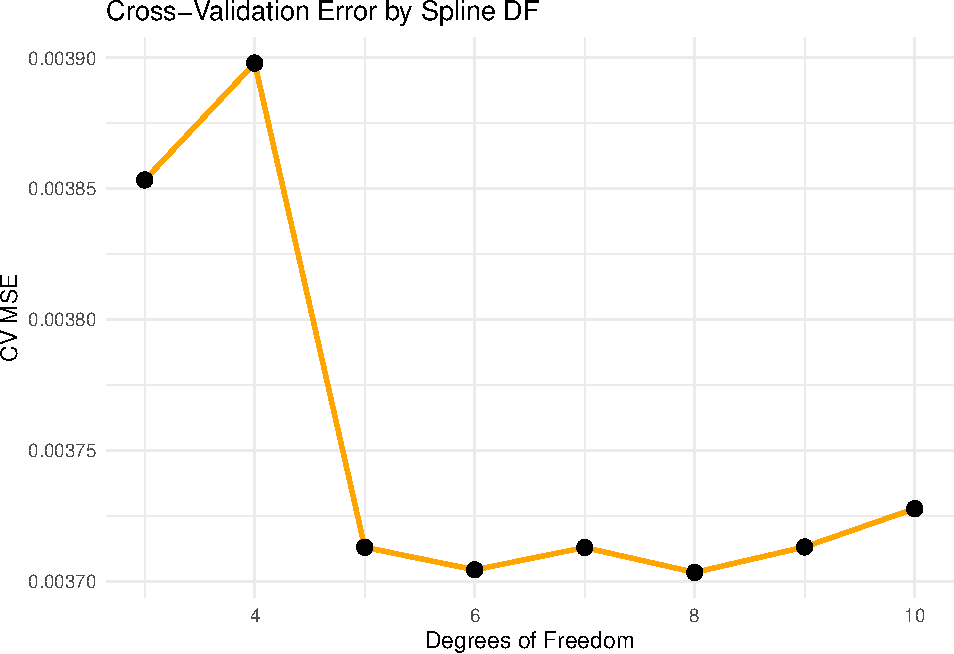
\includegraphics{chapter-07-hw_files/figure-latex/unnamed-chunk-9-1.pdf}

10-X cross-validation was performed to select the optimal degrees of
freedom for the regression spline. It reaches its lowest mean‑squared
error at \(df =8\), suggesting that an eight‑degree‑of‑freedom spline
offers the best bias--variance trade‑off, with \(df=7 \text{ or }9\)
performing nearly as well.

\end{document}
